\section{Aufbau und Versuchsdurchführung}

Die Versuchsdurchführung unterteilt sich in zwei Teilabschnitte. Zunächst wird ein Verfahren zur Unterdrückung von Störspannungen untersucht. Diese treten dann auf, wenn besonders kleine Signalspannungen mit Ausgangsklemmen abgegriffen werden.
Bei der Untersuchung von kleinen Brückenspannungen treten also Störspannungen auf die möglichst herausgefiltert werden müssen, da sie meistens die Ausgangsspannung völlig überdecken. Zunächst wird also eine Filterung des Störsignals mit
einem Selektivverstärker betrachtet.

\subsection{Bestimmung der Filterkurve eines Selektivverstärkers}
In dem Versuch werden ausschließlich monofrequente Eingangsspannungen verwendet welche an einem Selektivverstärker der Güte $Q = 20$ gefiltert werden. Zur Bestimmung der Filterkurve wird eine Ausgangsspannung eines Spannungsgenerators 
an einen Selektivverstärker angeschlossen und anschließend mit einem Millivoltmeter ausgelesen. 
Bei den für den zweiten Teil interessanten Brückenspannungen handelt es sich um sehr kleine Spannungswerte, deshalb verstärkt der Selektivverstärker das Signal um das 10-fache.
Nun werden Sinusspannungsfrequenzen $f$ zwischen $\SI{12}{}$-$\SI{35}{\kilo\hertz}$ in den Selektivverstärker gespeist und die resultierende Ausgangsspannung gemessen.
Die verwendete Spannunng des Spannungsgenerators konnte bei dem verwendeten Versuchsaufbau nicht abgelesen werden, diese ergibt sich allerdings bei der Auswertung des Maximums der Filterkurve durch die 10-fache Verstärkung des Selektivverstärkers.

\subsection{Messung der Suszeptibilitäten von Seltenen Erden} 
Für diesen Versuchsteil wird eine Brückenschaltung, wie in Abbildung .... gezeigt, mit einem Sinusspannungsgenerator verbunden, welcher auf die Frequenz $f$ eingestellt wird, bei der der Selektivverstärker zuvor sein Maximum hatte. Diese Frequenz beträgt hier $f = \SI{23}{\kilo\hertz}$.
Die Brückenspannungen lässt sich nun abgreifen, durch den Selektivverstärker mit 10-facher Verstärkung filtern und anschließend über ein Millivoltmeter auslesen. Hierbei wird weiterhin die gleiche Güte von $Q = 20$ verwendet.
Eine schematische Skizze des Aufbaus ist in Abbildung \ref{fig:aufbaumessung} dargestellt, jedoch wurde der Linearverstärker welcher vor dem Selektivverstärker gezeigt ist nicht verwendet.

\begin{figure}
    \centering
    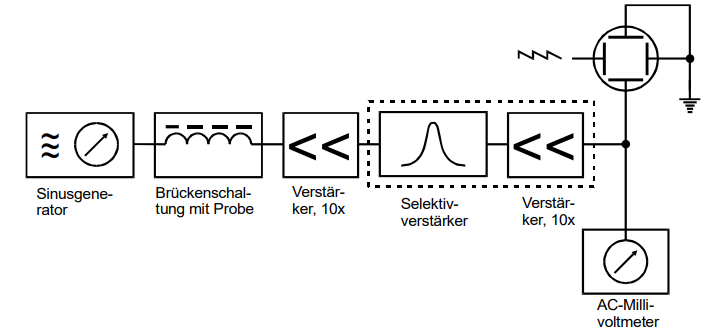
\includegraphics[width=\textwidth]{bilder/aufbaumessung.png}
    \caption{Schematische Skizze der einzelnen Schaltungselemente zur Messung der paramagnetischen Suszeptibilitäten. \cite{skript}} 
    \label{fig:aufbaumessung}
\end{figure}

An der Brückenschaltung gibt es zum ein Potentiometer, womit sich der Widerstand $R3$/$R4$ wie in Abbildung ... gezeigt regeln lässt, sowie einen Regelwiderstand $R_{p}$. Die Abmessungen der verwendeten Messspule sind in der Tabelle ... notiert. 
Untersucht werden insgesamte drei verschiedene Metallionen der seltenen Erden. Dazu gehören Gadolinium $\ce{Gd2O3}$, Dysprosium $\ce{Dy2O3}$ und Neodym $\ce{Nd2O3}$. Die Messproben dieser Stoffe werden zunächst mit einem Maßband gemessen und es wird ein Ablesefehler von
$\increment l= \SI{1}{\milli\meter}$ berücksichtigt. 
\\
\newline
Für die Bestimmung der Suszeptibilität durch die zwei beschriebene Methoden in \ref{sec:....} wird nun bei konstanter Eingangsspannung folgendes durchgeführt. 
Zunächst wird die Brückenspannung $U_{\text{BR}}$ so gut wie es geht abgeglichen. Dazu werden an der Brückenschaltung das Potentiometer $R3$/$R4$ und der Regelwiderstand so eingestellt, dass das Millivoltmeter ein Minimum anzeigt. Es wird jeweils die Brückenspannungen und der
Widerstand am Potentiometer notiert. 
\\
Nun wird eine Probe in die Spule der Brückenschaltung eingeführt, dabei muss darauf geachtet werden, dass die Probe nicht zu lange in der Hand gehalten wird damit sich die Temperatur von Spule und Probe nicht zu stark unterscheiden. Durch die 
veränderte Induktivität misst man nun eine Brückenspannung. Diese ist für die Auswertung ebenfalls von Interesse. Nun wird die Schaltung mitsamt der Probe wieder abgeglichen und der Widerstand des Potentiometers $R3$/$R4$ aufgeschrieben. Für
jede einzelne Probe wird dies dreimal wiederholt.